\begin{figure}[H]
    \centering
    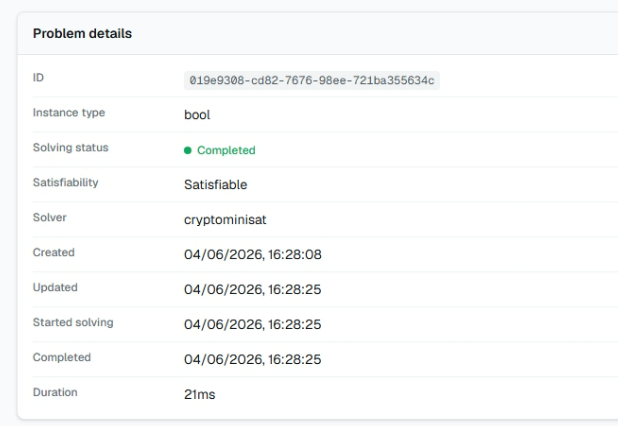
\includegraphics[width=\textwidth]{img/e2e-01-1.png}
    \caption{E2E-01 \ref{sec:testing:e2e-01}: Detail problému Boolovej formuly \texttt{((x -> y) + x) * y <-> false}}
    \label{fig:e2e-01-01}
\end{figure}

\begin{figure}[H]
    \centering
    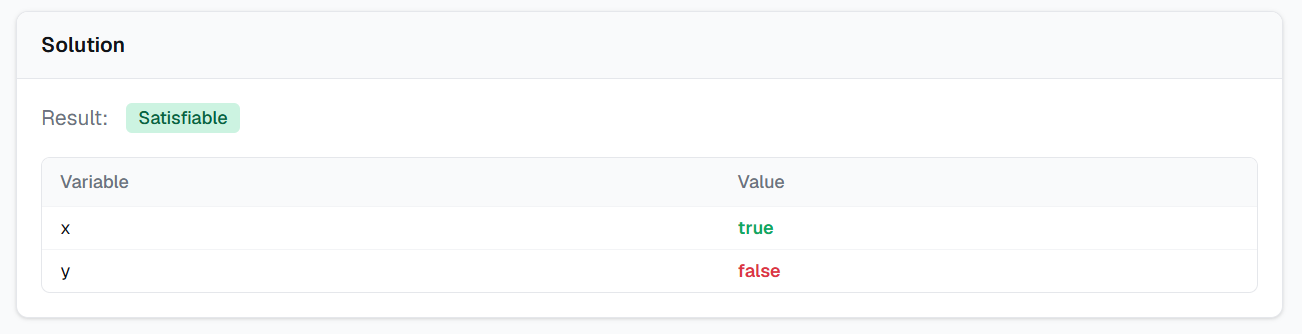
\includegraphics[width=\textwidth]{img/e2e-01-2.1.png}
    \caption{E2E-01 \ref{sec:testing:e2e-01}: Riešenia Boolovej formuly \texttt{((x -> y) + x) * y <-> false}}
    \label{fig:e2e-01-02}
\end{figure}

\begin{figure}[H]
    \centering
    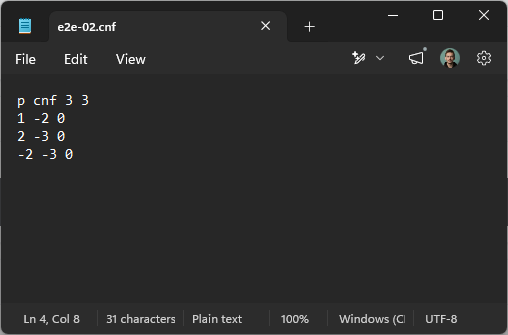
\includegraphics[width=\textwidth]{img/e2e-02-1.png}
    \caption{E2E-02 \ref{sec:testing:e2e-02}: Súbor na nahratie}
    \label{fig:e2e-02-01}
\end{figure}

\begin{figure}[H]
    \centering
    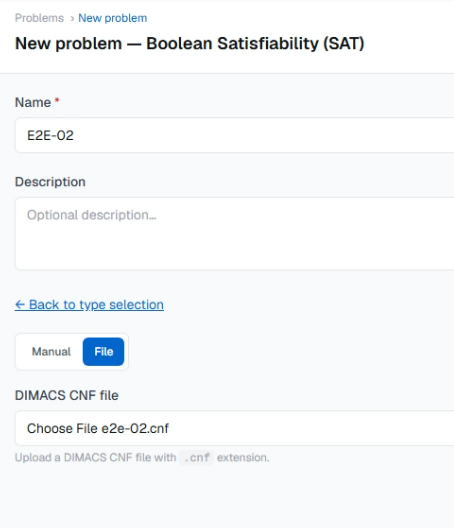
\includegraphics[width=\textwidth]{img/e2e-02-2.png}
    \caption{E2E-02 \ref{sec:testing:e2e-02}: Formulár s načítanou \acrshort{sat} inštanciou}
    \label{fig:e2e-02-02}
\end{figure}

\begin{figure}[H]
    \centering
    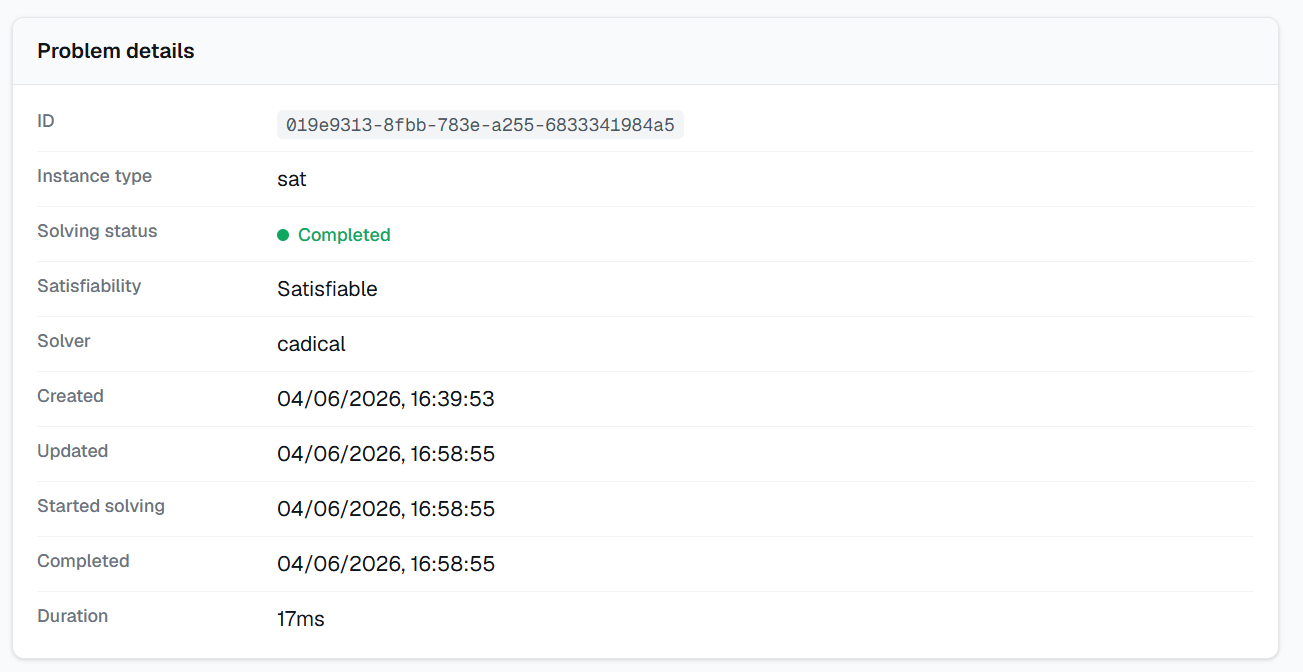
\includegraphics[width=\textwidth]{img/e2e-02-3.1.1.png}
    \caption{E2E-02 \ref{sec:testing:e2e-02}: Detail problému \acrshort{sat} inštancie}
    \label{fig:e2e-02-03-01}
\end{figure}

\begin{figure}[H]
    \centering
    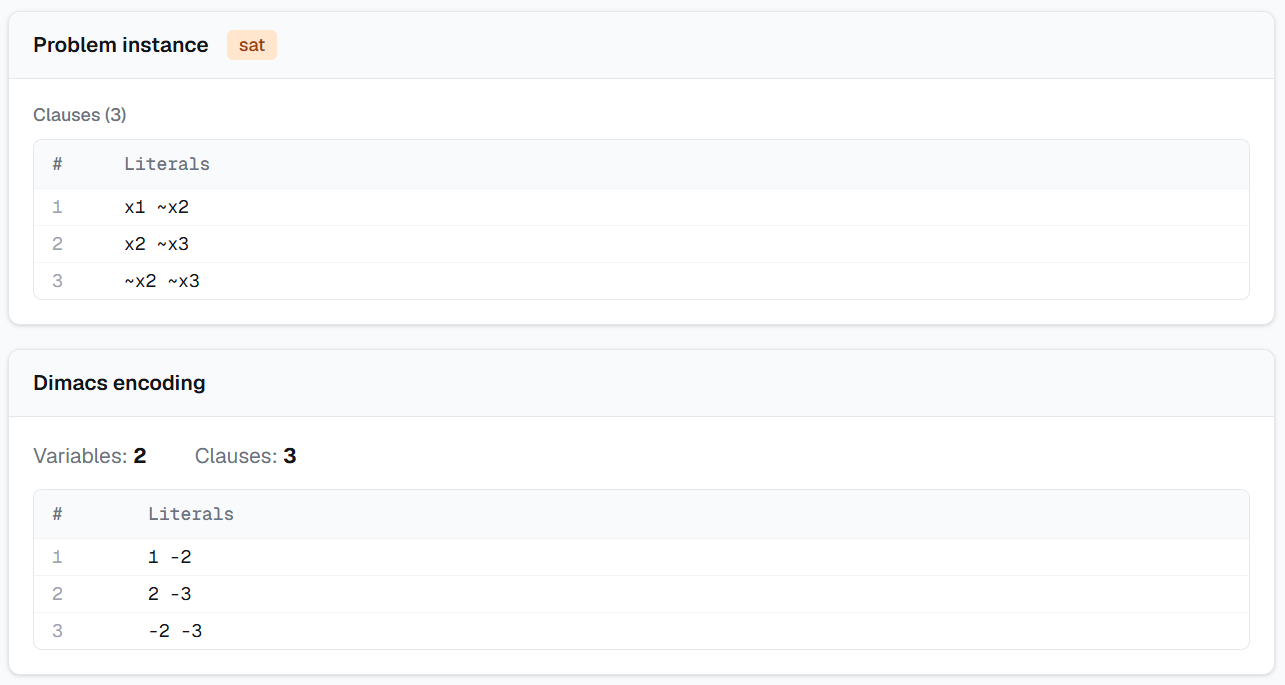
\includegraphics[width=\textwidth]{img/e2e-02-3.2.png}
    \caption{E2E-02 \ref{sec:testing:e2e-02}: Inštancia \acrshort{sat} z číselným DIMACS kódovaním}
    \label{fig:e2e-02-03-02}
\end{figure}

\begin{figure}[H]
    \centering
    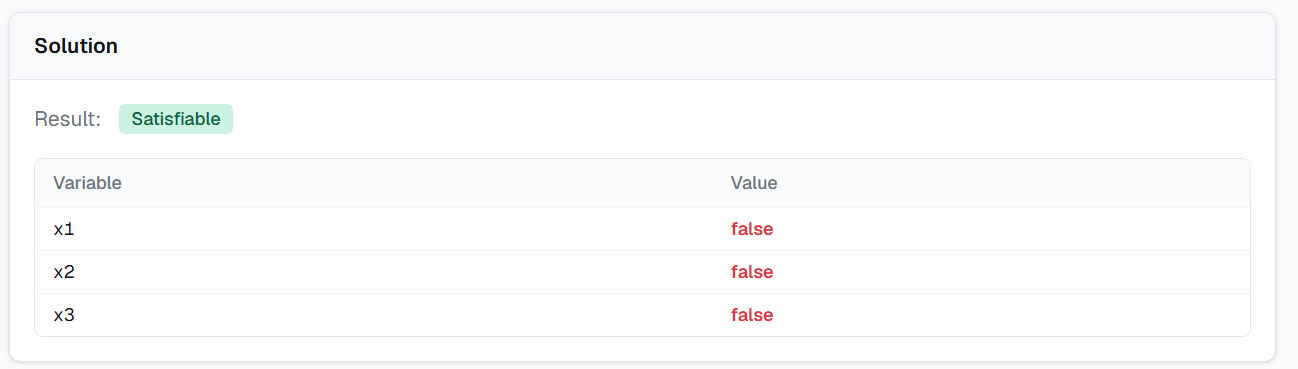
\includegraphics[width=\textwidth]{img/e2e-02-3.3.png}
    \caption{E2E-02 \ref{sec:testing:e2e-02}: Riešenia \acrshort{sat} inštancie}
    \label{fig:e2e-02-03-03}
\end{figure}

\begin{figure}[H]
    \centering
    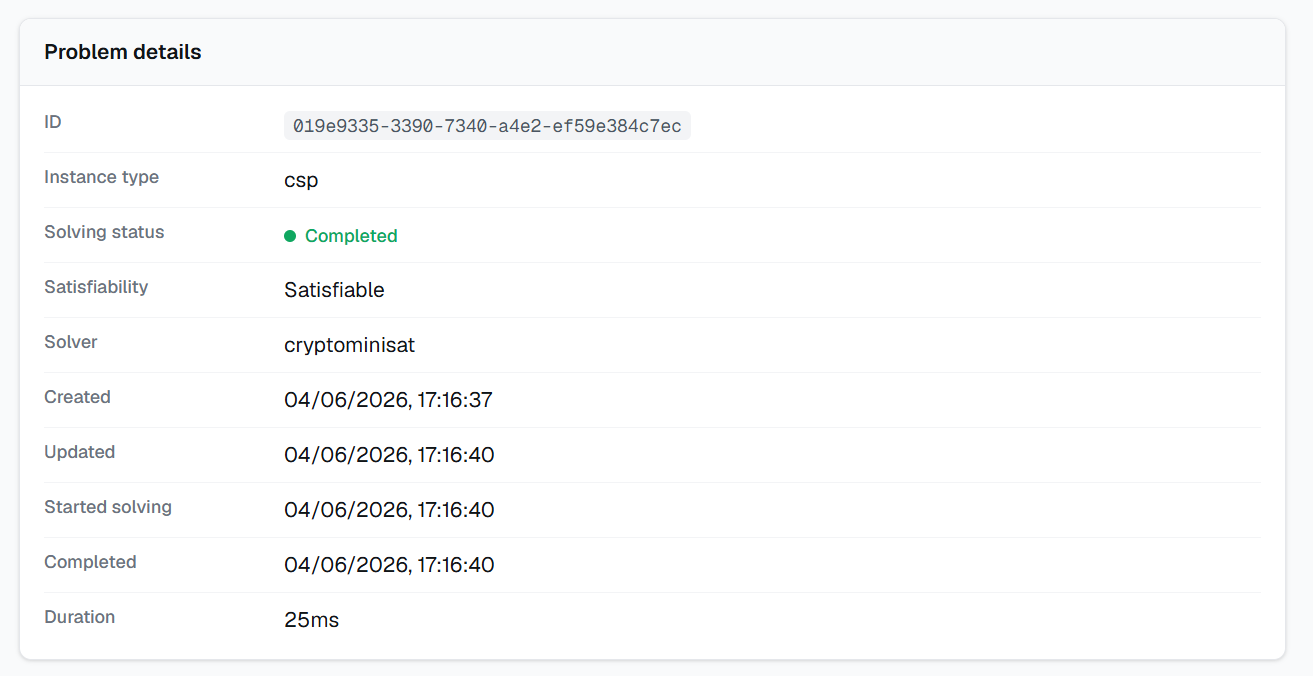
\includegraphics[width=\textwidth]{img/e2e-03-1.1.png}
    \caption{E2E-03 \ref{sec:testing:e2e-03}: Detail problému \acrshort{csp} inštancie}
    \label{fig:e2e-03-01-01}
\end{figure}

\begin{figure}[H]
    \centering
    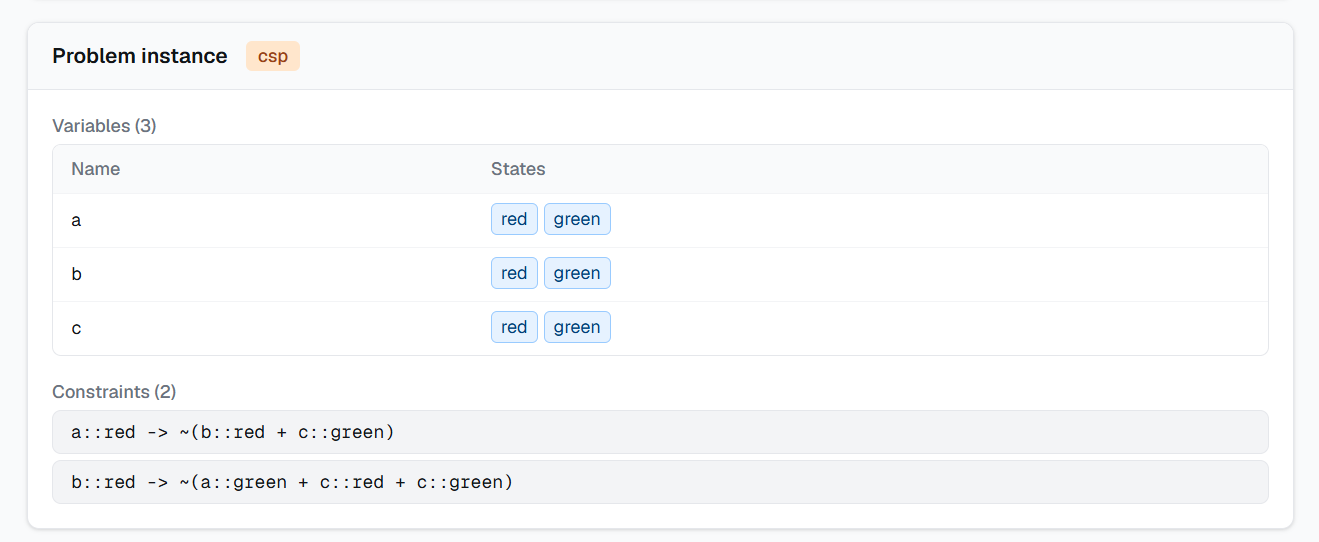
\includegraphics[width=\textwidth]{img/e2e-03-2.1.png}
    \caption{E2E-03 \ref{sec:testing:e2e-03}: Inštancia \acrshort{csp}}
    \label{fig:e2e-03-02-01}
\end{figure}

\begin{figure}[H]
    \centering
    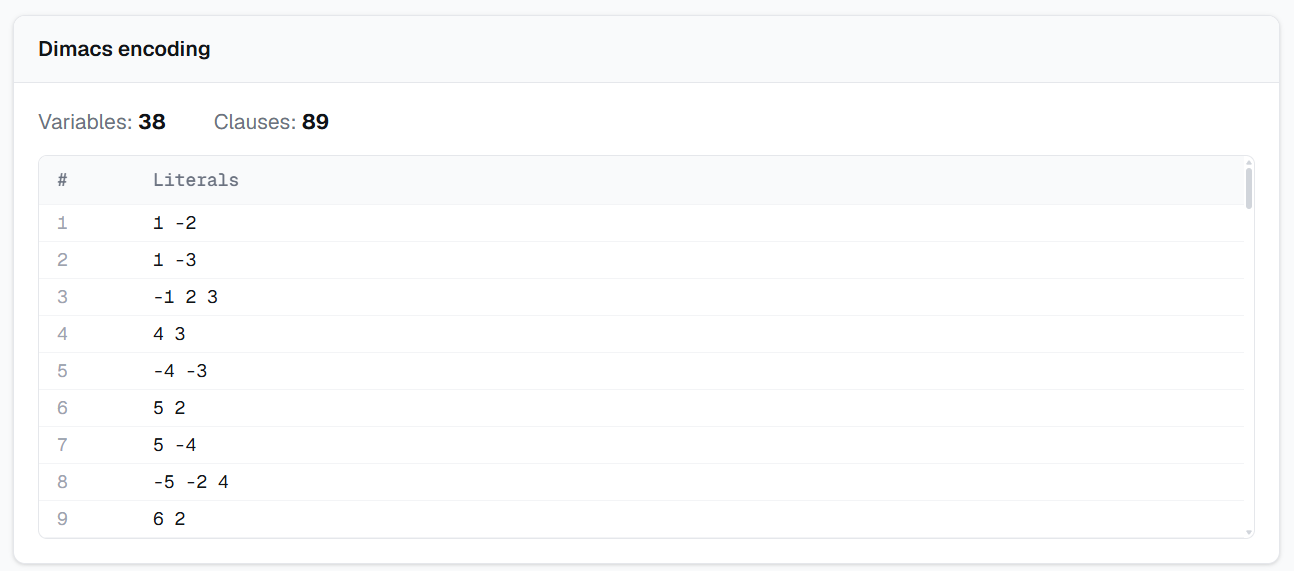
\includegraphics[width=\textwidth]{img/e2e-03-3.1.png}
    \caption{E2E-03 \ref{sec:testing:e2e-03}: Začiatok DIMACS kódovania \acrshort{csp} inštancie}
    \label{fig:e2e-03-03-01}
\end{figure}

\begin{figure}[H]
    \centering
    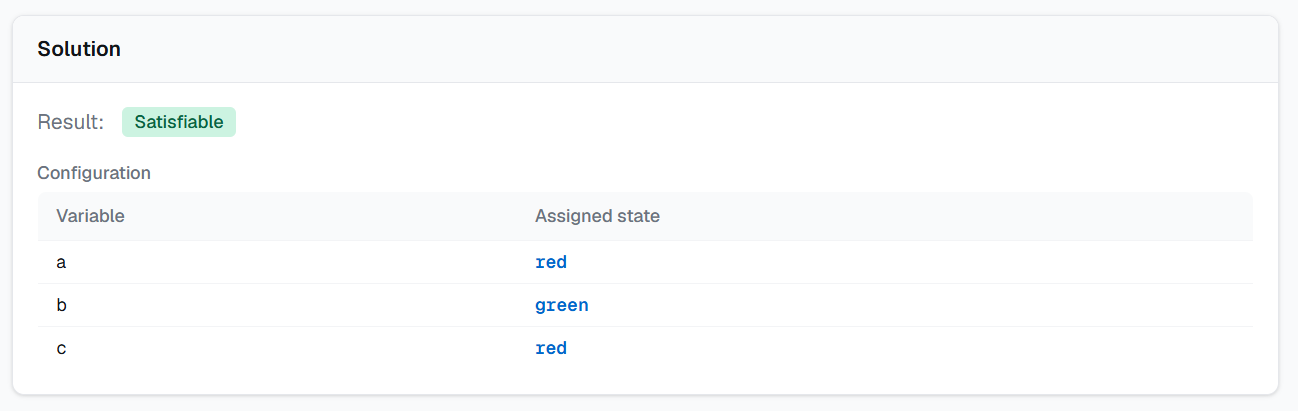
\includegraphics[width=\textwidth]{img/e2e-03-4.1.png}
    \caption{E2E-03 \ref{sec:testing:e2e-03}: Riešenia \acrshort{csp} inštancie}
    \label{fig:e2e-03-04-01}
\end{figure}

\begin{figure}[H]
    \centering
    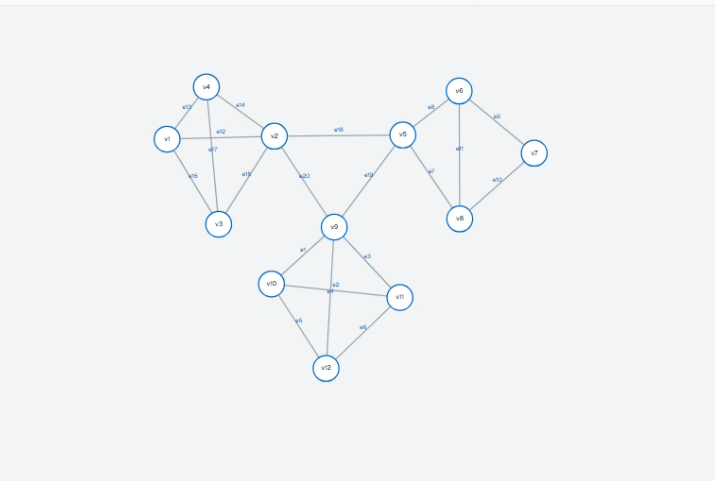
\includegraphics[width=\textwidth]{img/e2e-04-1.png}
    \caption{E2E-04 \ref{sec:testing:e2e-04}: Zadanie grafu na vrcholové farbenie (počet farieb je 4)}
    \label{fig:e2e-04-01}
\end{figure}

\begin{figure}[H]
    \centering
    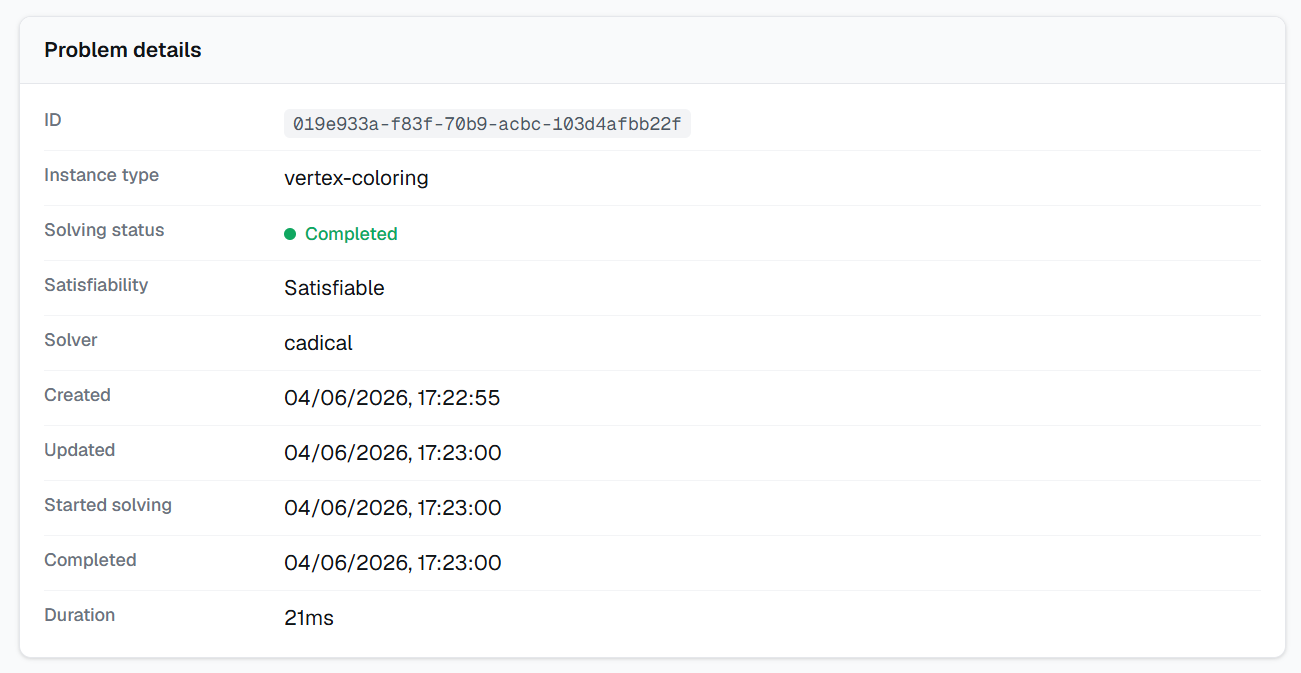
\includegraphics[width=\textwidth]{img/e2e-04-1.1.png}
    \caption{E2E-04 \ref{sec:testing:e2e-04}: Detail problému vrcholového farbenia grafu}
    \label{fig:e2e-04-02}
\end{figure}

\begin{figure}[H]
    \centering
    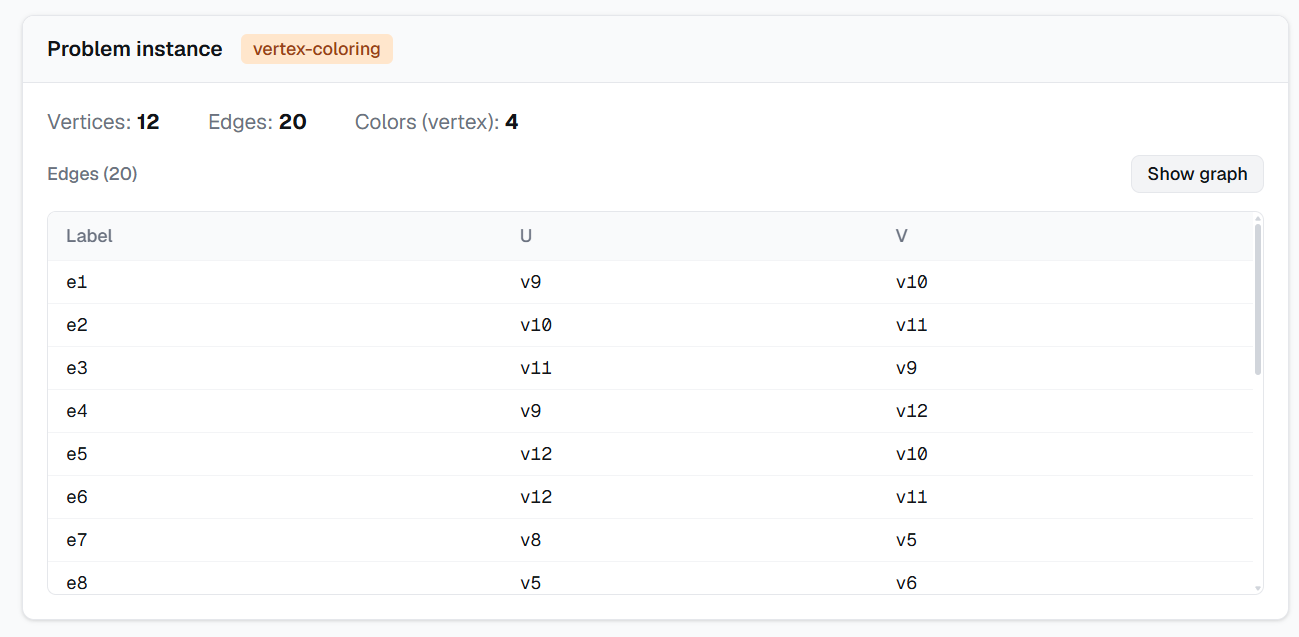
\includegraphics[width=\textwidth]{img/e2e-04-2.1.png}
    \caption{E2E-04 \ref{sec:testing:e2e-04}: Začiatok inštancie problému vrcholového farbenia grafu}
    \label{fig:e2e-04-02-01}
\end{figure}

\begin{figure}[H]
    \centering
    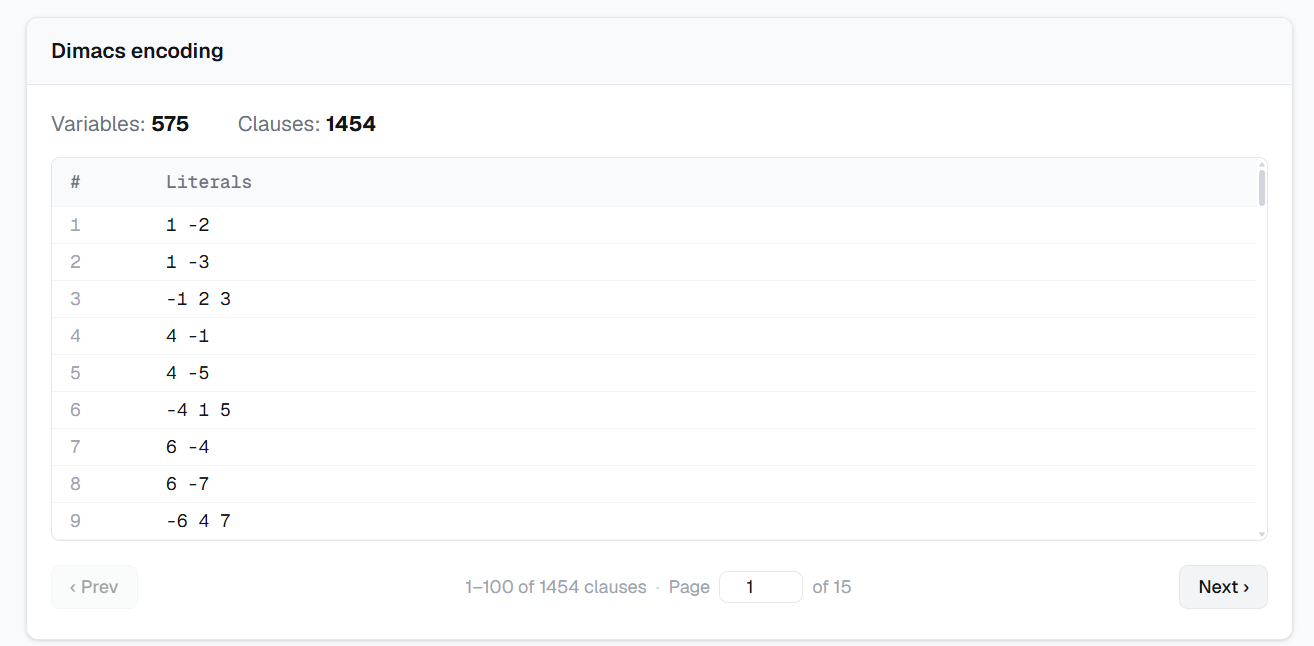
\includegraphics[width=\textwidth]{img/e2e-04-3.1.png}
    \caption{E2E-04 \ref{sec:testing:e2e-04}: Začiatok DIMACS kódovania problému vrcholového farbenia grafu}
    \label{fig:e2e-04-03-01}
\end{figure}

\begin{figure}[H]
    \centering
    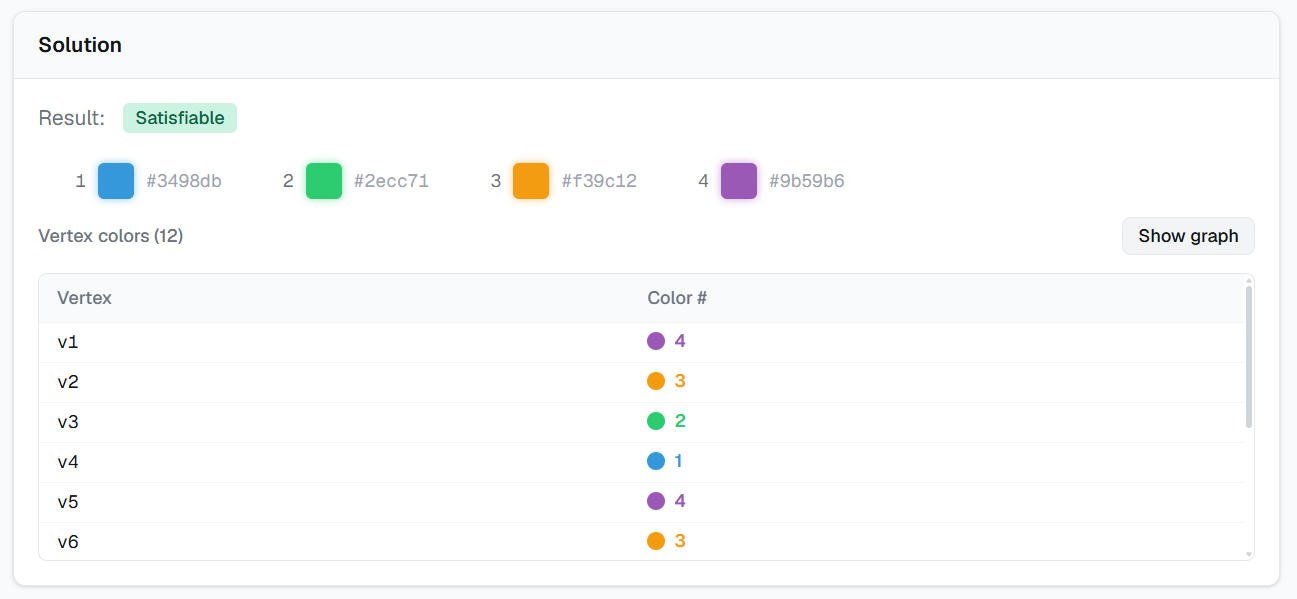
\includegraphics[width=\textwidth]{img/e2e-04-4.1.png}
    \caption{E2E-04 \ref{sec:testing:e2e-04}: Začiatok riešenia problému vrcholového farbenia grafu}
    \label{fig:e2e-04-04-01}
\end{figure}

\begin{figure}[H]
    \centering
    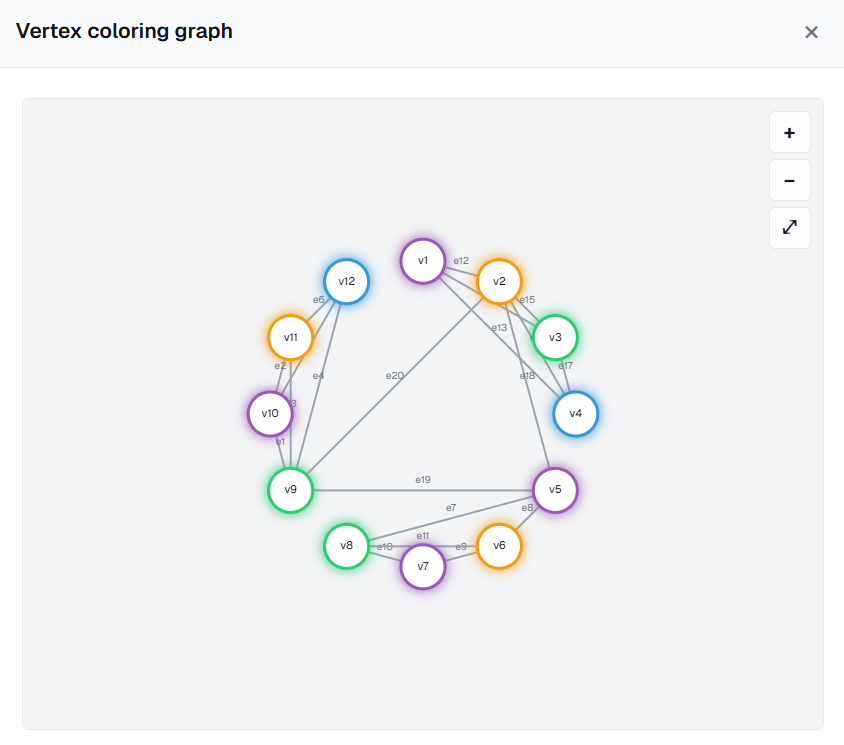
\includegraphics[width=\textwidth]{img/e2e-04-5.png}
    \caption{E2E-04 \ref{sec:testing:e2e-04}: Vizualizácia riešenia problému vrcholového farbenia grafu}
    \label{fig:e2e-04-05}
\end{figure}

\begin{figure}[H]
    \centering
    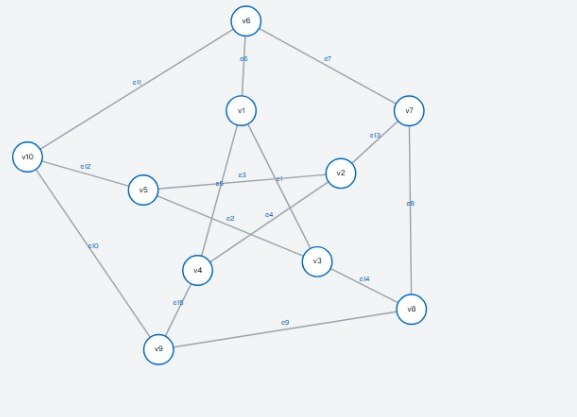
\includegraphics[width=\textwidth]{img/e2e-05-1.png}
    \caption{E2E-05 \ref{sec:testing:e2e-05}: Zadanie grafu na hranové farbenie (Peterson graf; počet farieb je 4)}
    \label{fig:e2e-05-01}
\end{figure}

\begin{figure}[H]
    \centering
    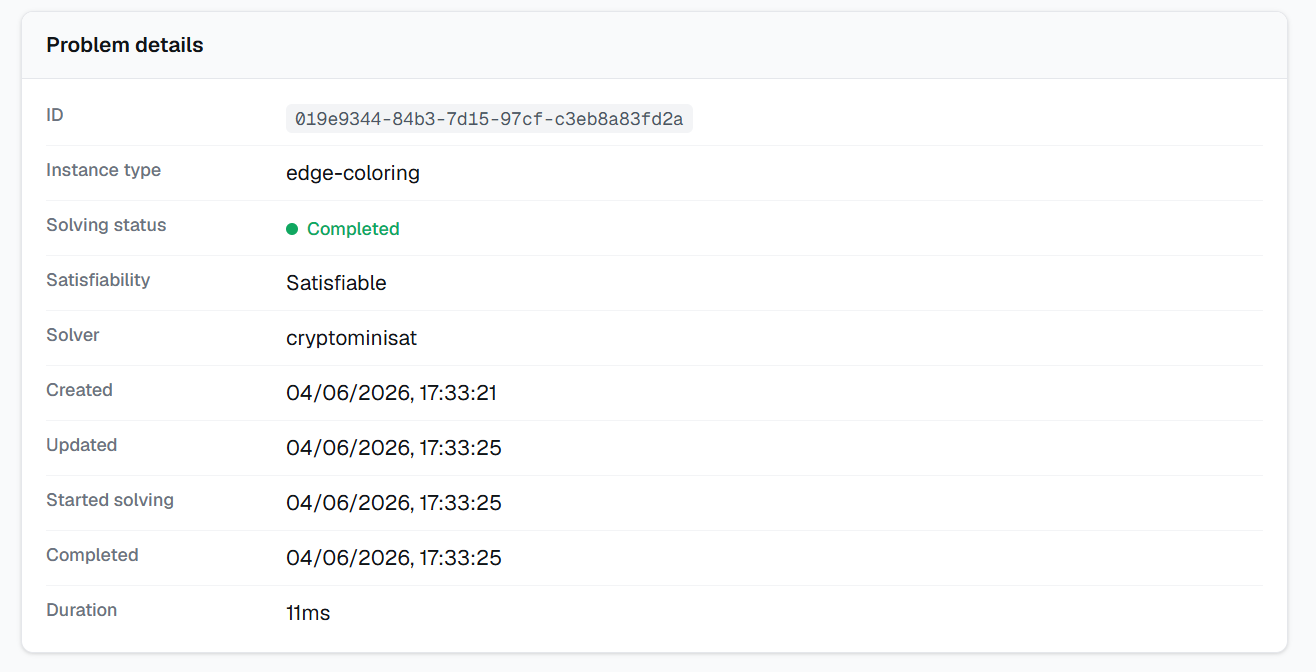
\includegraphics[width=\textwidth]{img/e2e-05-2.1.png}
    \caption{E2E-05 \ref{sec:testing:e2e-05}: Detail problému hranového farbenia grafu}
    \label{fig:e2e-05-02-01}
\end{figure}

\begin{figure}[H]
    \centering
    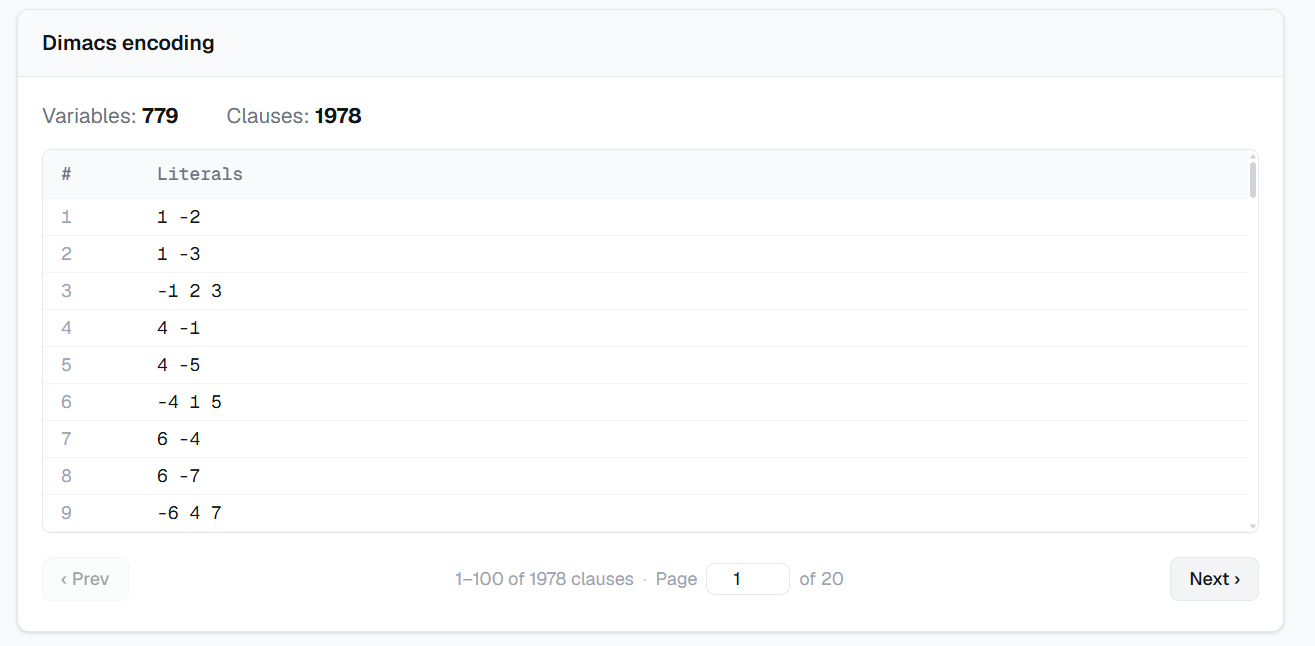
\includegraphics[width=\textwidth]{img/e2e-05-3.1.png}
    \caption{E2E-05 \ref{sec:testing:e2e-05}: Začiatok DIMACS kódovania problému hranového farbenia grafu}
    \label{fig:e2e-05-03-01}
\end{figure}

\begin{figure}[H]
    \centering
    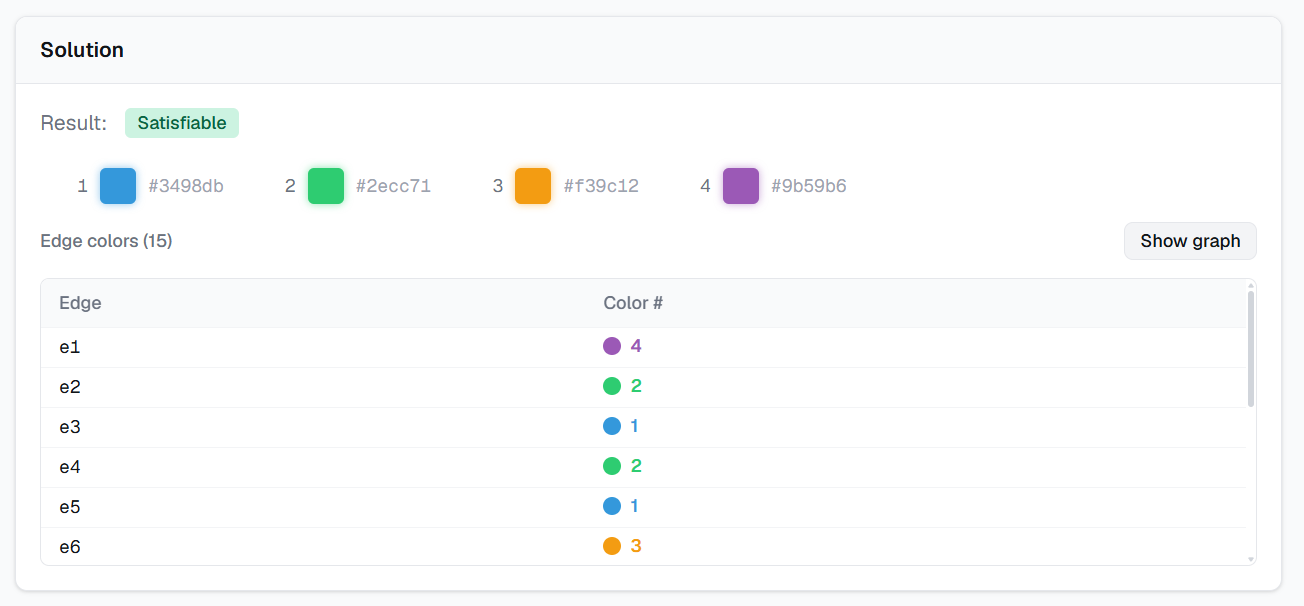
\includegraphics[width=\textwidth]{img/e2e-05-4.1.png}
    \caption{E2E-05 \ref{sec:testing:e2e-05}: Začiatok riešenia problému hranového farbenia grafu}
    \label{fig:e2e-05-04-01}
\end{figure}

\begin{figure}[H]
    \centering
    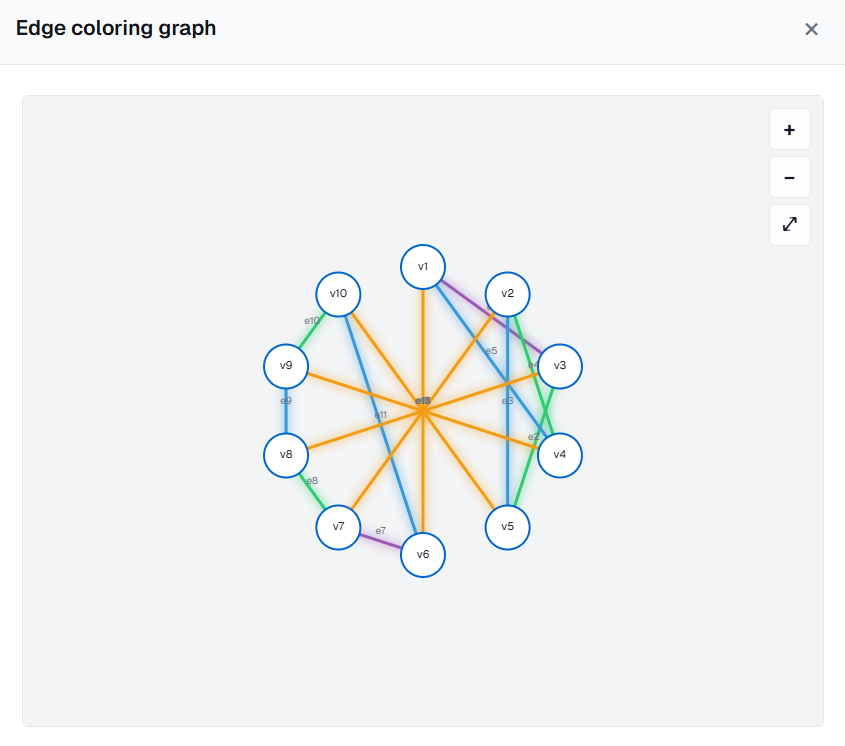
\includegraphics[width=\textwidth]{img/e2e-05-5.png}
    \caption{E2E-05 \ref{sec:testing:e2e-05}: Vizualizácia riešenia problému hranového farbenia grafu}
    \label{fig:e2e-05-05}
\end{figure}

\begin{figure}[H]
    \centering
    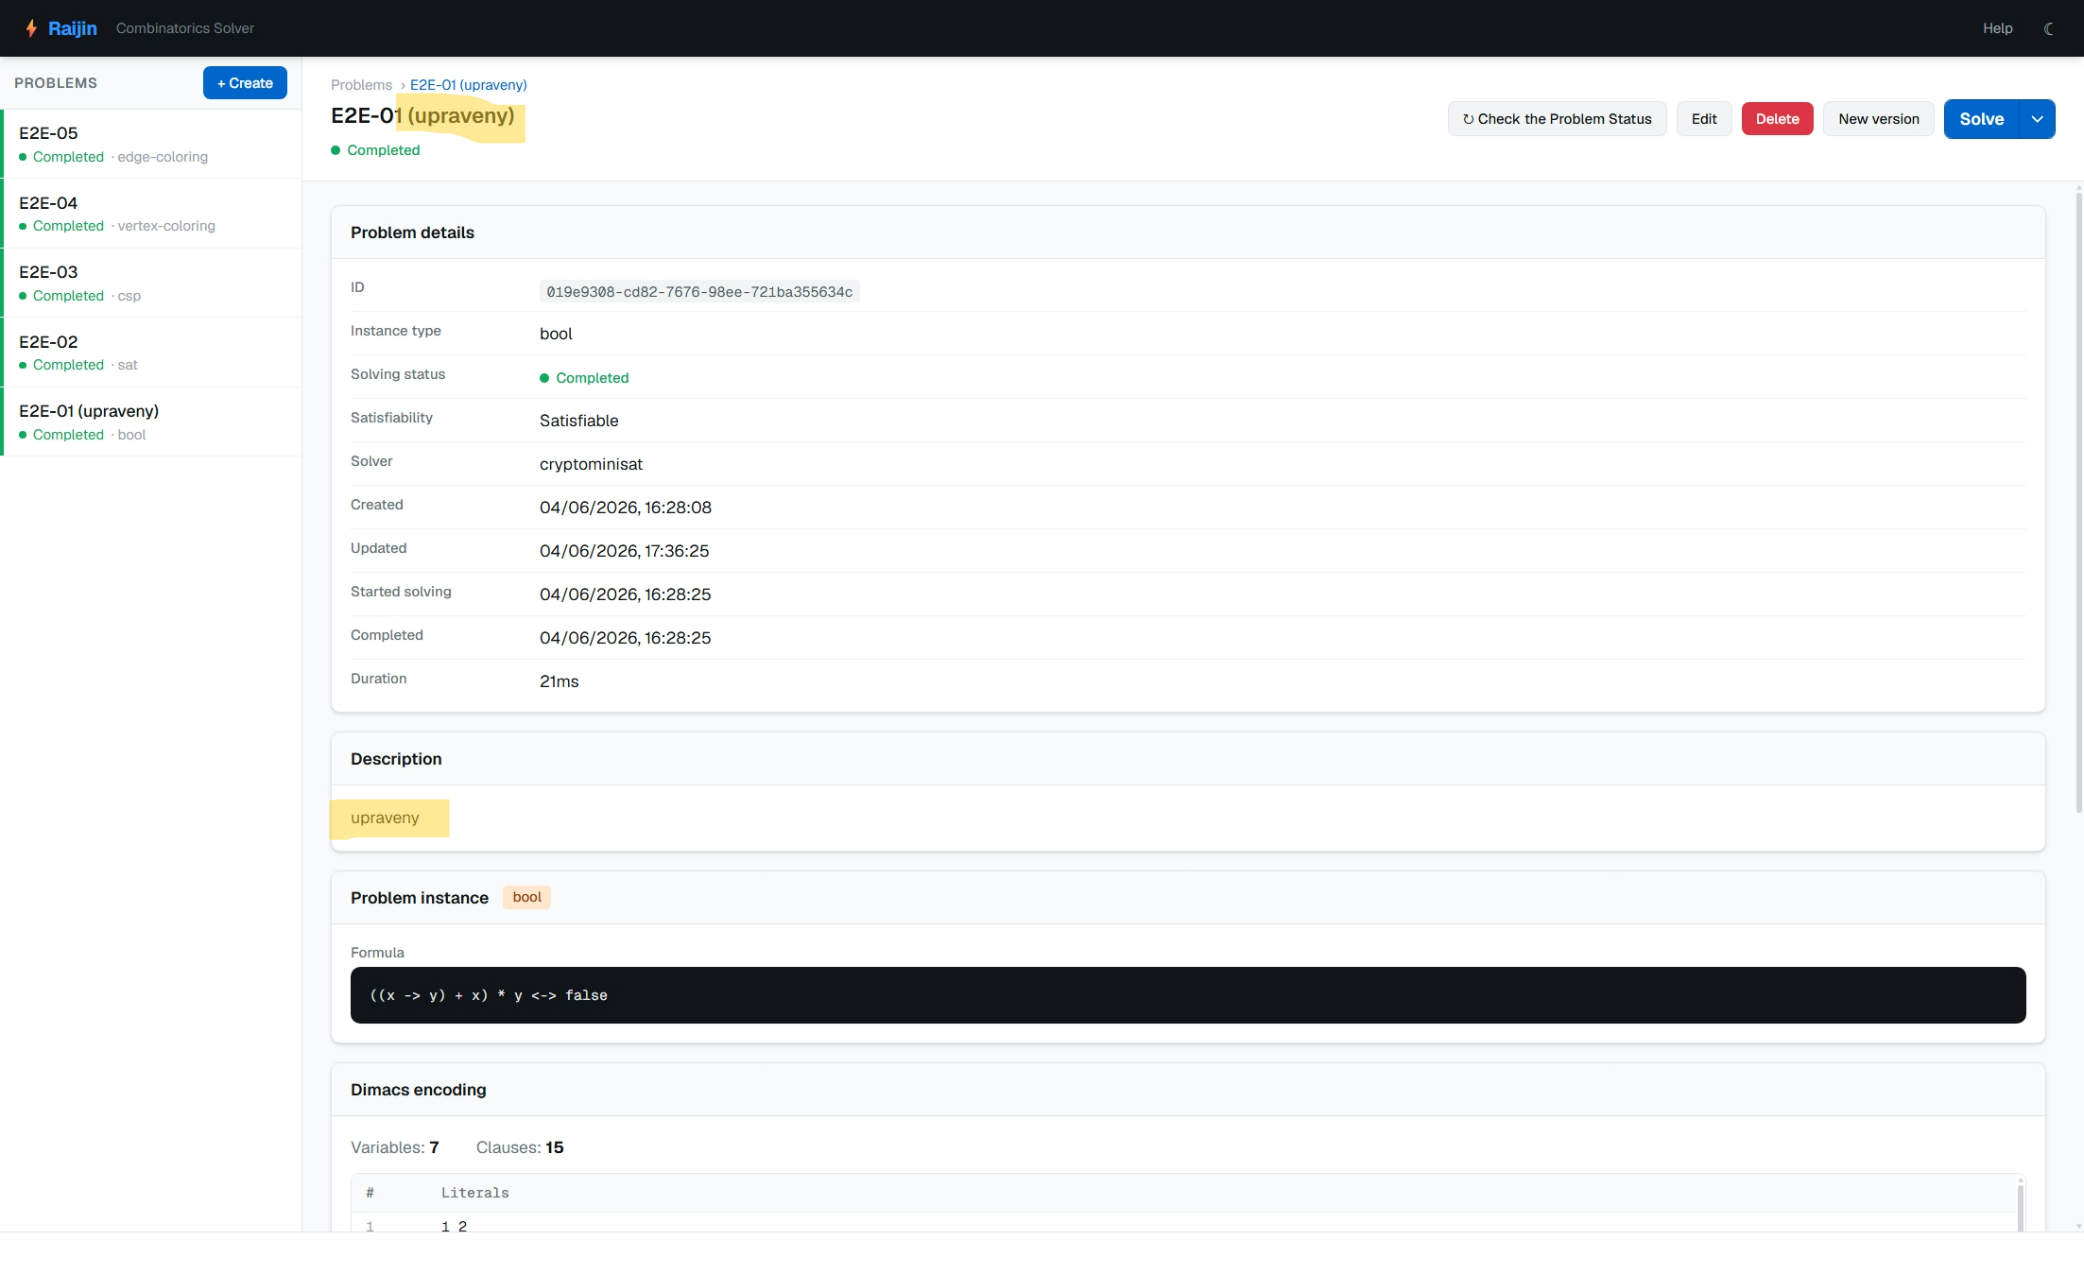
\includegraphics[width=\textwidth]{img/e2e-06-1.png}
    \caption{E2E-06 \ref{sec:testing:e2e-06}: Upravený problém}
    \label{fig:e2e-06-01}
\end{figure}

\begin{figure}[H]
    \centering
    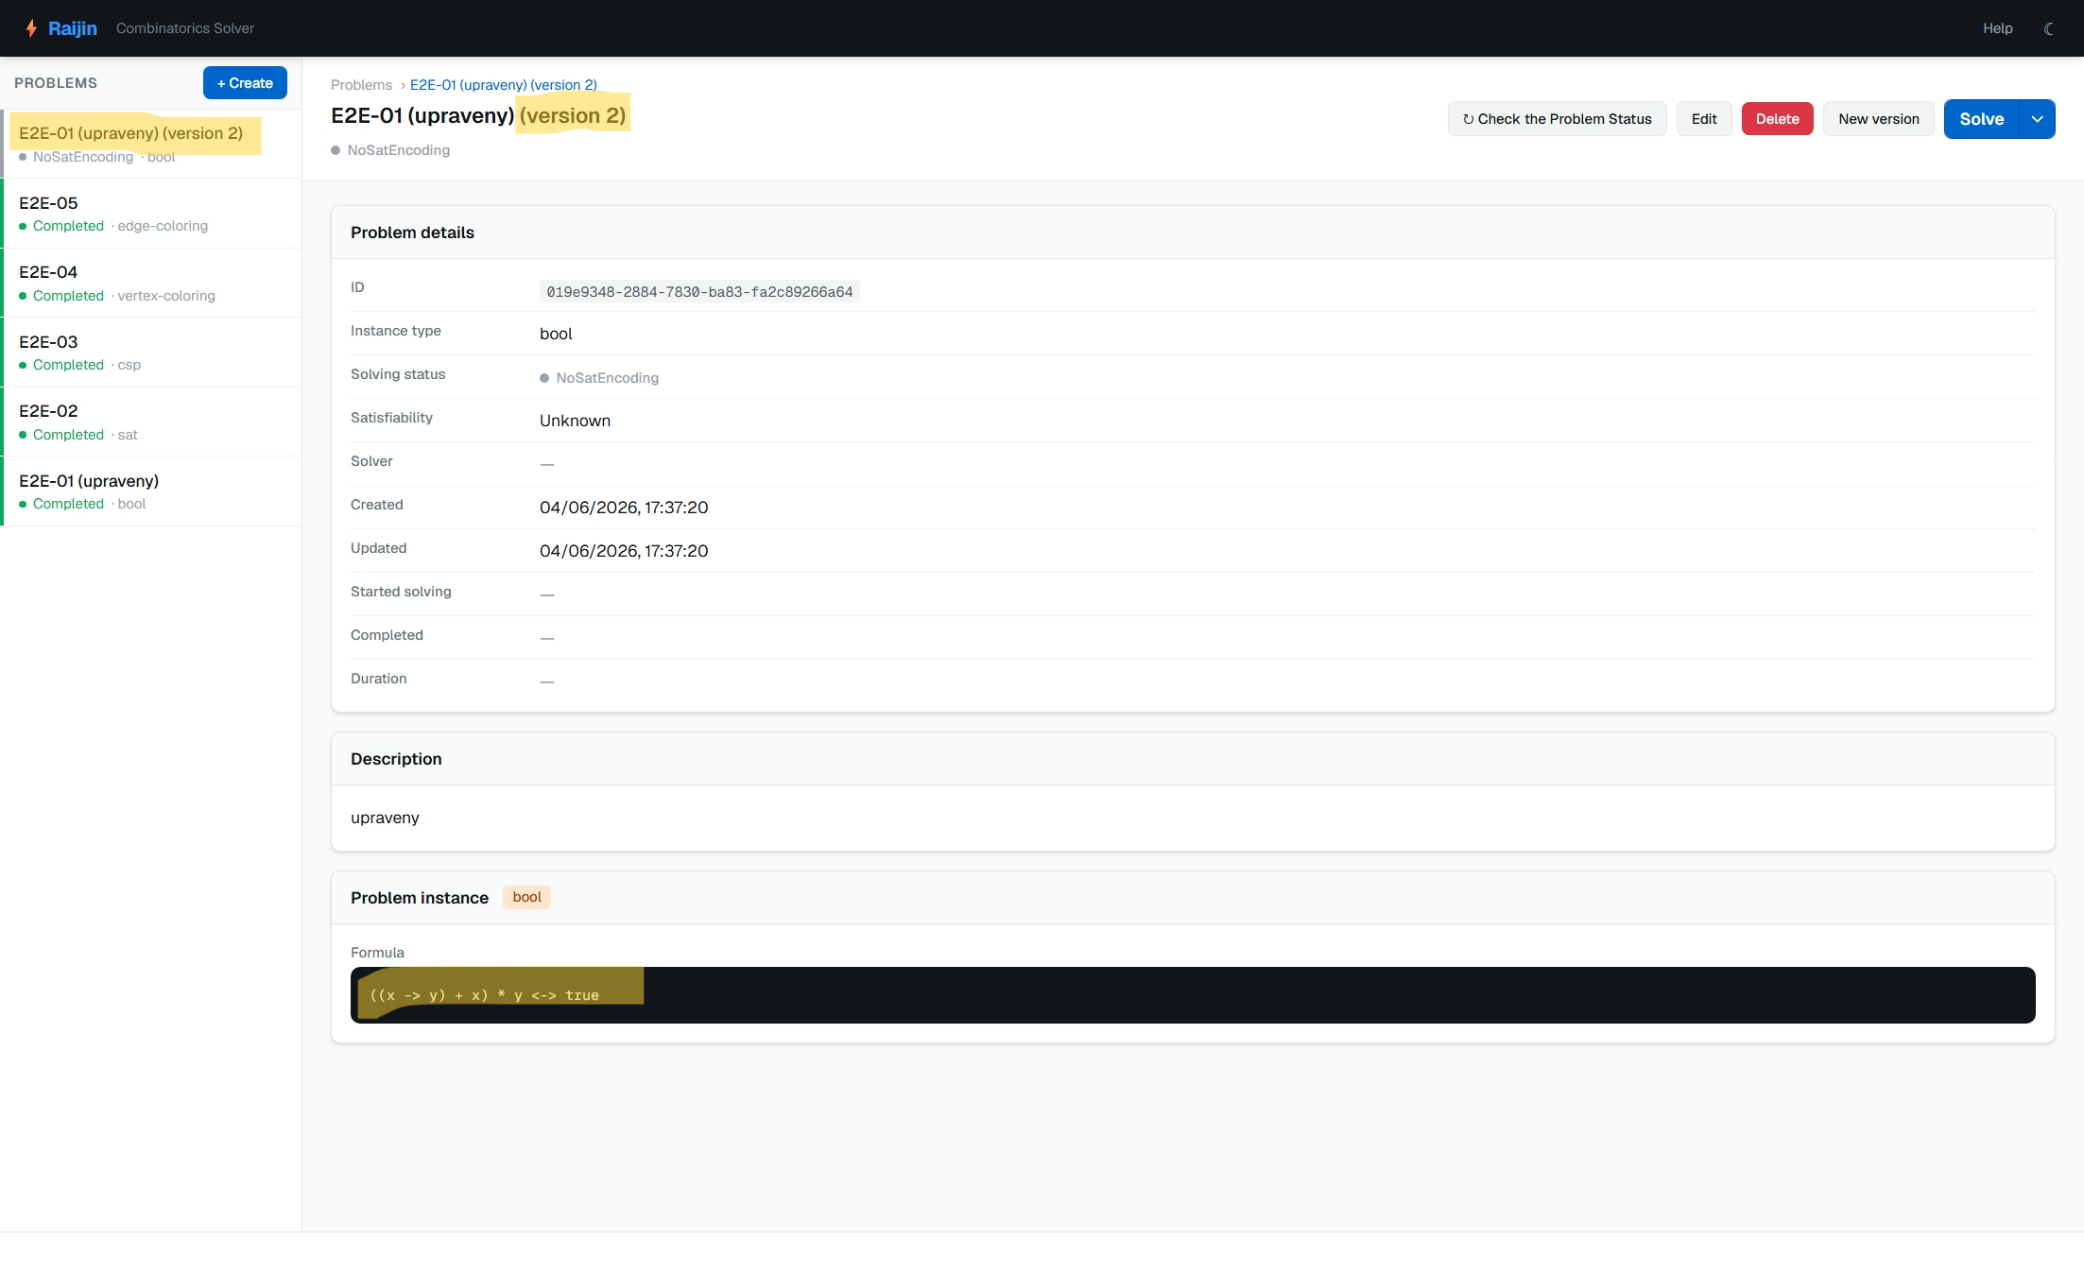
\includegraphics[width=\textwidth]{img/e2e-06-2.png}
    \caption{E2E-06 \ref{sec:testing:e2e-06}: Nová verzia problému}
    \label{fig:e2e-06-02}
\end{figure}

\begin{figure}[H]
    \centering
    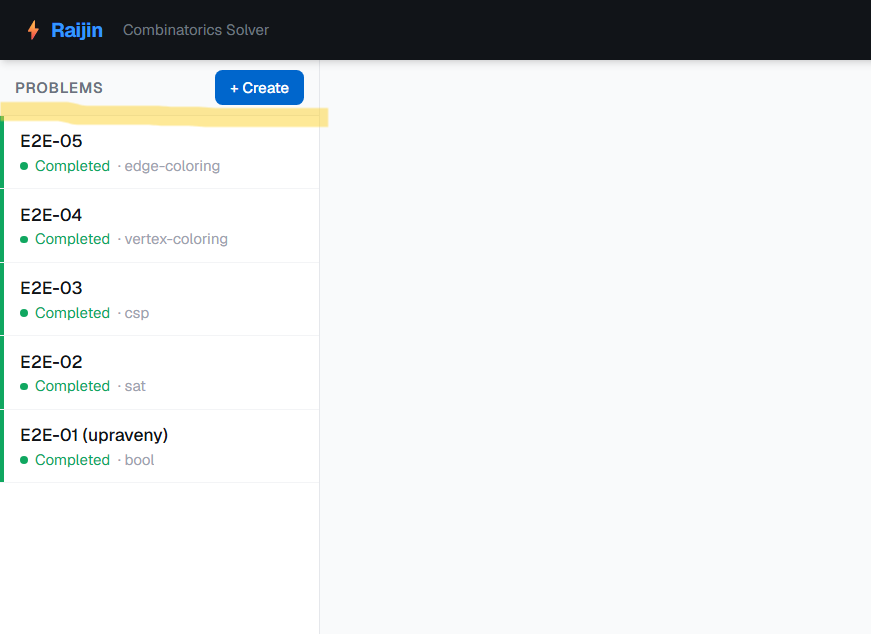
\includegraphics[width=\textwidth]{img/e2e-06-3.png}
    \caption{E2E-06 \ref{sec:testing:e2e-06}: Zoznam problémov po odstránení novej verzie problému}
    \label{fig:e2e-06-03}
\end{figure}

\begin{figure}[H]
    \centering
    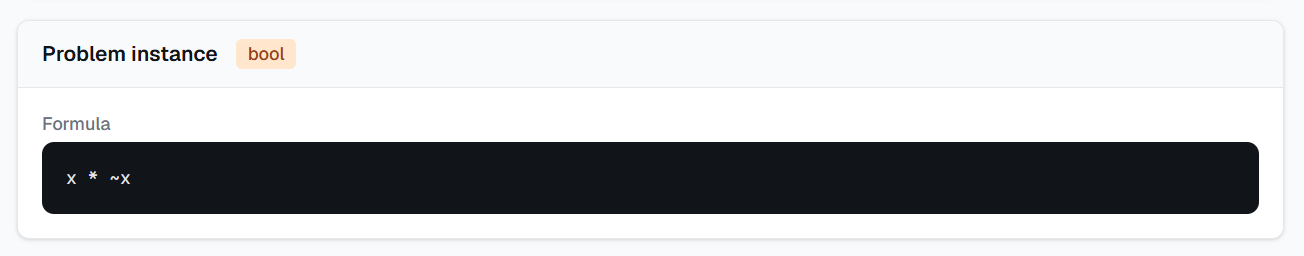
\includegraphics[width=\textwidth]{img/e2e-07-1.1.png}
    \caption{E2E-07 \ref{sec:testing:e2e-07}: Vytvorený nesplniteľný problém}
    \label{fig:e2e-07-01}
\end{figure}

\begin{figure}[H]
    \centering
    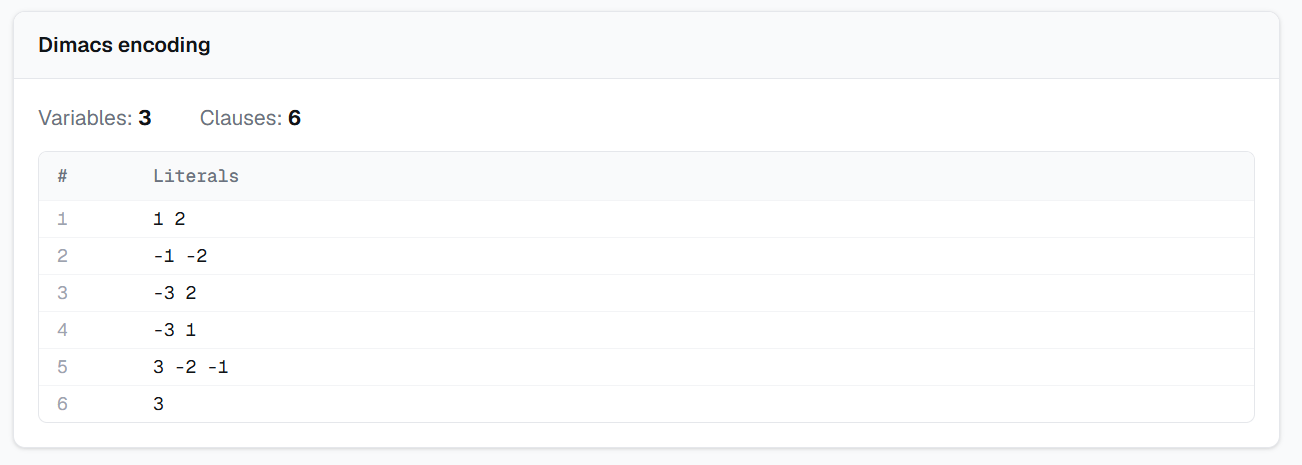
\includegraphics[width=\textwidth]{img/e2e-07-2.1.png}
    \caption{E2E-07 \ref{sec:testing:e2e-07}: DIMACS kódovania nesplniteľného problému}
    \label{fig:e2e-07-02}
\end{figure}

\begin{figure}[H]
    \centering
    
\includegraphics[width=\textwidth]{img/e2e-07-3.1.png}
    \caption{E2E-07 \ref{sec:testing:e2e-07}: Riešenia nesplniteľného problému}
    \label{fig:e2e-07-03}
\end{figure}
